\scanpage{16}
\mspage{30}

\deleted{\deleted{pourra alors}\inserted{\unsure{faut donc}}
\deleted{\unsure{respecter}}\inserted{dans 3.9.} l'hypothèse \deleted{dans 3.9.}
avec : ``ou \deleted{\unsure{$B$ est lui-même un corps}}\inserted{$r(B)=r(A)B$}''
\deleted{(car grâce au résultat du et la}}

\uline{Corollaire} \inserted{4.}10. Soient $A$ un anneau local noethérien, de corps résiduel
$k$, $B_0$ une $k$-algèbre qui soit un anneau local noethérien, et soit une $k$-algèbre
de Cohen i.e. une $k$-algèbre formellement simple \deleted{pour sa} et complète
pour sa topologie ordinaire. Supposons de plus l'extension résiduelle $K/k$
séparable (ce qui n'est donc pas une restriction si $B_0=K$\deleted{\unsure{fini}}, mais en est
évidemment une en général). Alors il existe une $A$-algèbre topologique de
Cohen \inserted{$B$} qui se réduit suivant $B_0$, $B$ est unique à isomorphisme près
en vertu de \inserted{4.}8., et c'est un anneau noethérien local complet comme il se doit.

En vertu du théorème de structure \inserted{3.}4. on a $B_0\simeq K[[T_1,\ldots,T_n]]$,
et on est ramené, grâce au critère \inserted{4.}9. 2) et la transitivité de la
platitude, aux deux cas types: 1°) $B_0=K$ 2°) $B_0=k[[T_1,\ldots,T_n]]$. Dans
le premier cas, on utilise le résultat général de $0_{\mathrm{III}}$\inserted{10.3.1.}, et dans le
deuxième cas il suffit de prendre $B=\widehat{A}[[T_1,\ldots,T_n]]$.

\deleted{Théorème 3.1} \uline{Corollaire} \inserted{4.}11. Sous les conditions de 3.9.,
\inserted{si $k(B)/k(A)$ de multi. rad. finie,}
les conditions 1) et 2) équivalent aussi à: 3) $B$ est complet et formellement simple sur $A$

En effet, on sait déjà que \deleted{c'est nécessaire,}\inserted{$1)\longrightarrow3)$}
reste à prouver \deleted{la} $3)\Longrightarrow1)$
\deleted{suffisance} ou encore $3)\Longrightarrow2)$, i.e. on est ramené à prouver simplement que
$B$ est plat sur $A$. Or\unsure{n} faisant une extension de la base $A\longrightarrow A'$, $A'$ local
libre \inserted{de type fini} sur $A$ à extension radicielle convenable (cf $0_{\mathrm{III}}$), on trouve un $B'$
\inserted{local} sur $A'$ qui sera encore formellement simple sur $A'$, et de plus à extension
résiduelle \deleted{triviale} séparable. On dispose alors du théorème d'existence
\inserted{4.}10. qui nous garantit, grâce à \inserted{4.}8. (équiv de 0) et 1) ) que $B'$ est
Cohen sur $A'$ donc plat sur $A'$. Donc $B$ est plat sur $A$.

\margin{\figure{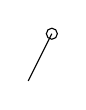
\begin{tikzpicture}\draw (0,0)--(.3,.6);\draw (.3,.6) circle (.07);\end{tikzpicture}}
(réduction \inserted{du NB} inutile dans le cas ``visé'')}

\mspage{15}
